% https://tex.stackexchange.com/q/715947/86
\documentclass[tikz,border=5pt]{standalone}
\usepackage[dvipsnames]{xcolor}
\usetikzlibrary{
  arrows.meta,
  shapes.misc,
  positioning,
  shapes.geometric,
  intersections,
  spath3
}%

\begin{document}

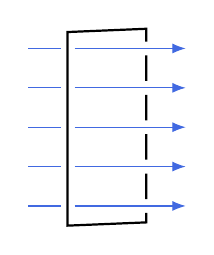
\begin{tikzpicture}[>=Latex]

% Create and save the arrow paths
\foreach \k in {1,...,5} {
    \path[
        spath/save global=b\k%
    ] (0,-1.5 + \k/2) -- ++(2,0);
}

% Create the trapezium shape
\node[
    trapezium,%
    rotate=90,
    minimum width = 2.5cm,
    minimum height= 1cm,
    trapezium left angle = 100,
    trapezium right angle = 80,
    trapezium stretches=true,
    trapezium stretches body =true,
    spath/save global=trap1%设置全局路径
] (t) at (1,0) {};

% Split the trapezium and each of the arrows where they meet,
% then insert gaps in the arrow paths at one of the intersections,
% then remove the split in the arrow paths where we didn't insert a gap.
\foreach \k in {1,...,5} {
    \tikzset{
        spath/split globally at intersections={trap1}{b\k},
        spath/insert gaps globally after components={b\k}{5pt}{1},
        spath/spot weld globally={b\k},
    }
}

% % This inserts the gaps in the trapezium path, we make an alias style
% % just to shorten the code.
\tikzset{
    do stuff/.style={
        spath/insert gaps after components={trap1}{5pt}{#1},
    },
    do stuff/.list={5,6,7,8,9},
}

% % Now render the arrow paths
\foreach \k in {1,...,5} {
    \draw[spath/use=b\k,->,RoyalBlue];
}

% % Now render the trapezium path
\draw[black,thick,spath/use=trap1];

\end{tikzpicture}
\end{document}